\documentclass[a4paper,10pt]{report}
\usepackage[utf8]{inputenc}
\usepackage{geometry, amsmath, amsthm, latexsym, amssymb, graphicx}
\usepackage{hyperref}
\usepackage{gensymb}

\usepackage{environ}
\usepackage{tabto,enumitem}
\usepackage{lipsum}

\title{The arccosine function}
\author{Himansi Patel - 40072262}

\begin{document}



\section{The arccosine function}
\subsection{Description}

The arccosine function is the inverse trigonometric function.\\
The arccosine of x is defined as the inverse cosine function of x when -1$\leq$x$\leq$1.
When the cosine of y is equal to x:
\begin{equation}
\cos y = x
\end{equation}
Then the arccosine of x is equal to the inverse cosine function of x, which is equal to y:
\begin{equation}
\arccos x = \cos^-1 x = y 
\end{equation}
(Here $\cos^-1$ x means the inverse cosine and does not mean cosine to the power of -1).\cite{rapidtables}\\
For example,\\
\begin{minipage}{0.30\textwidth}
    \centering
    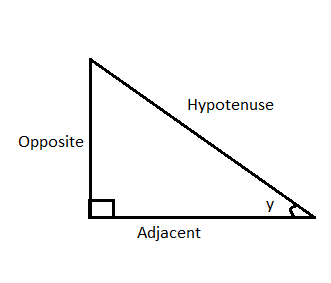
\includegraphics[width=\textwidth]{Firstpic.PNG}
    \end{minipage}
    \begin{minipage}{0.70\textwidth}
    \begin{equation}
\cos y = \frac{Adjacent}{Hypotenuse} \rightarrow y=\arccos(\frac{Adjacent}{Hypotenuse})
\end{equation}
    \end{minipage}

\subsection{Domain \& Co-Domain of arccosine}
\begin{itemize}[noitemsep]
\item The domain of $\arccos x $ is  -1 $\leq$ x $\leq$ 1.
\item The range of $\arccos x $ is  0 $\leq$ y $\leq$ $\pi$ in radians or $0^{\circ}$$\leq$ y $\leq$$180^{\circ}$ in degrees.
\item It is most useful when trying to find the angle measure when two sides of a triangle are known.
\end{itemize}

\subsection{Properties of arccosine}
    \begin{minipage}{0.40\textwidth}
    \centering
    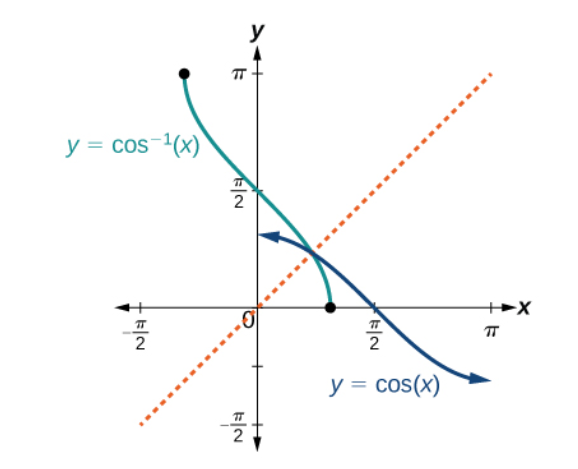
\includegraphics[width=\textwidth]{Capturelast.PNG}
    \end{minipage}
    \begin{minipage}{0.60\textwidth}
    \begin{itemize}[noitemsep]
      \item For the arccosine function to be a true inverse function of the sine function, the following statement must be true$\colon$ $\cos(\arccos(x))=x$ and $\arccos(\cos(x))=x$
      \item The arccosine function is a reflection of the cosine function about the line $y=x$.
      \item The arccosine function is defined when -1 $\leq$ x $\leq$1
      \item The arccosine function is continuous on open interval (-1,1)
      
    \end{itemize}
    \end{minipage}

\subsection{Application of arccosine}
\begin{itemize}[noitemsep]
\item Arccosine function are unique function and useful in finding remaining angles of right triangle.
\item It is also useful in application of engineering, physics and others.
\end{itemize}


\begin{thebibliography}{9}
\bibitem{lumenlearning}
\url{https://courses.lumenlearning.com/boundless-algebra/chapter/trigonometric-functions-and-the-unit-circle/}
\bibitem{rapidtables}
\url{https://www.rapidtables.com/math/trigonometry/arccos.html}
\end{thebibliography}


\end{document}
